\newcommand{\kvad}{kvadratne funkcije}

\subsubsection{Domena i kodomena \kvad}
    Kvadratna funkcije je polinomna funkcija drugog stupnja. Najčešće ju srecemo u sljedećem obliku:
    \[f(x) = ax^2 + bx + c,\; a \neq 0\]
    \(x\) je argument funkcije, \(a\) zovemo kvadratni koeficijent, \(b\) zovemo linearni koeficjient, a \(c\) slobodni koeficjient.
    Možemo ju naći i u faktoriziranom obliku:
    \[f(x) = a(x - x_1)(x - x_2)\]

\subsubsection{Graf \kvad}
    Graf kvadratne funkcija zove se parabola.
    Ako je \(a > 0\) otvor je prema gore, a ako je \(a < 0\) otvor je prema dolje.
    Apsoultna vrijednost \(a\) određuje stupanj otvorenosti parabole tako da je parabola za manji a \emph{"uža"}.
    Tjeme je određeno koeficijentima \(a, b\) i \(c\):
    \[T(-\frac{b}{2a}, \frac{4ac - b^2}{4a})\]
    Slobodni koeficijent \(c\) određuje odsječak na y-osi.
    \begin{figure}[ht]
        \centering
        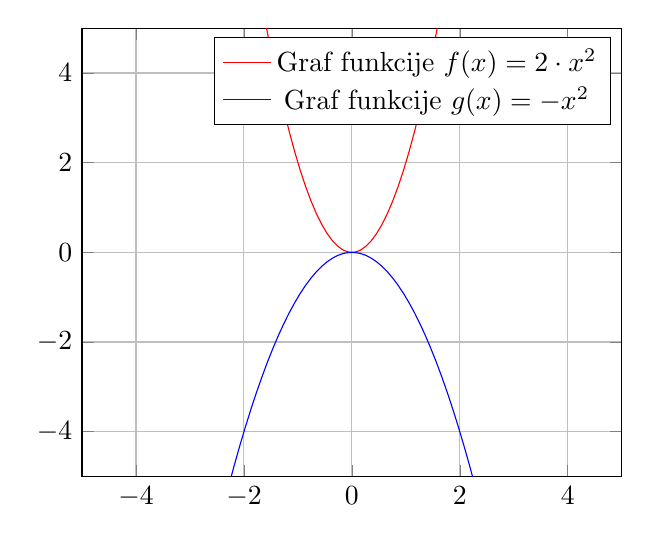
\begin{tikzpicture}
            \begin{axis}[
                grid=major,
                ymin=-5,
                ymax=5,
                xmin=-5,
                xmax=5,
            ]
                \addplot[
                    color = red,
                    samples = 100
                ]{2 * x^2};
                \addlegendentry{Graf funkcije \(f(x) = 2 \cdot x^2\)}
                \addplot[
                    color = blue,
                    samples = 100
                ]{-x^2};
                \addlegendentry{Graf funkcije \(g(x) = -x^2\)}
            \end{axis}
        \end{tikzpicture}
        \caption{Grafovi kvadratnih funkcija s različitim predznakom kvadratnim koeficijentom (vidi otvor i veličinu otvora)}
        \label{fig:template}
    \end{figure}
    \begin{figure}[ht]
        \centering
        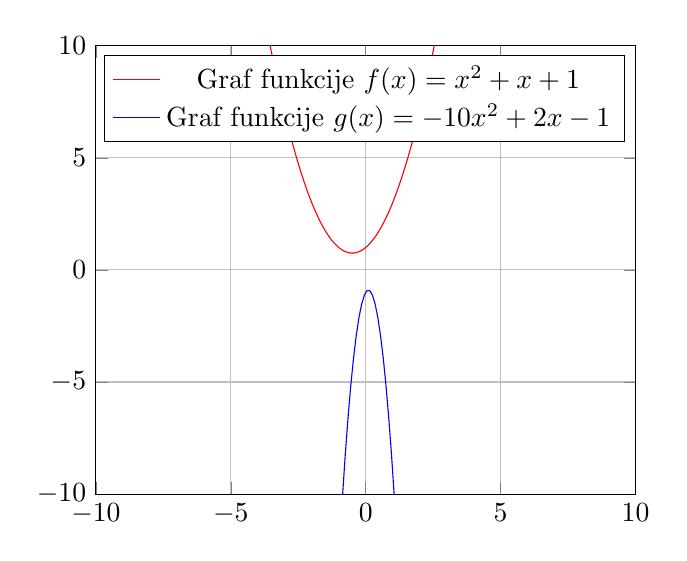
\begin{tikzpicture}
            \begin{axis}[
                grid=major,
                ymin=-10,
                ymax=10,
                xmin=-10,
                xmax=10,
            ]
                \addplot[
                    color = red,
                    samples = 100
                ]{x^2 + x + 1};
                \addlegendentry{Graf funkcije \(f(x) = x^2 + x + 1\)}
                \addplot[
                    color = blue,
                    samples = 100
                ]{-10 * x^2 + 2 * x - 1};
                \addlegendentry{Graf funkcije \(g(x) = -10x^2 + 2x - 1\)}
            \end{axis}
        \end{tikzpicture}
        \caption{Grafovi kvadratnih funkcija s različitim tjemenima}
        \label{fig:template}
    \end{figure}
    

\subsubsection{Nultočke i točke u kojima graf sječe y-os \kvad}
    Nultočke kvadratne funkcije pronalazimo formulom:
    \[x_{1, 2} = \frac{-b \pm \sqrt{b^2 - 4ac}}{2a}\]
    Nultočaka je \(0\), \(1\) ili \(2\) ovisno o diskriminanti \(D = \sqrt{b^2 - 4ac}\).
    Parabola y-os sječe u jednoj točki.

\subsubsection{Parnost i neparnost \kvad}
    Kvadratna funkcija je parnog stupnja pa je parna za \(b = 0\):
    \begin{equation*}
        \begin{split}
            f(x)            &= f(-x) \\
            ax^2 + bx + c   &= a(-x)^2 - bx + c \\
            ax^2 + bx + c   &= ax^2 - bx + c \\
            bx              &= - bx \\
            b               &= 0 
        \end{split}
    \end{equation*}
    Kvadratna funkcija nije neparna jer je parna a nije \(f(x) = 0\).
\subsubsection{Periodičnost \kvad}
    Kvadratna funkcija nije periodična, ne postoji \(P\) za koji vrijedi \(f(x + P) = f(x),\; P \neq 0\).

\subsubsection{Monotonost \kvad}
    Kvadratna funkcija nije monotona.
    Za \(a > 0\) do tjemena strogo pada, a od njega strogo raste, a za \(a < 0\) do tjemena strogo raste, a od njega strogo pada.

\subsubsection{Omeđenost \kvad}
    Kvadratna funkcija je omeđena tijemenom.

\subsubsection{Injektivnost i surjektivnost \kvad}
    Kvadratna funkcija nije injekcija:
    \begin{equation*}
        \begin{split}
            x_1 = 2,\; x_2 &= -2,\; f(x) = x^2 \\ 
            f(2) &= f(-2) \\
            4a &= 4a \\
            0& = 0
        \end{split}
    \end{equation*}
    \\
    Različiti argumenti nisu implicirali različite rezultate što je proturiječno s tvrdnjom u \ref{injekt}.
    Kvadratna funkcija je surjektivnost jer vrijedi tvrdnja u \ref{injekt}.

\subsubsection{Inverz \kvad}
    Kvadratna funkcija nema inverz jer je surjekcija (\ref{injekt}).
    Korijen je inverz kvadratne funkcije, ali samo na intervalu intervalu \(\mathbb{R}^+\).
    \begin{figure}[ht]
        \centering
        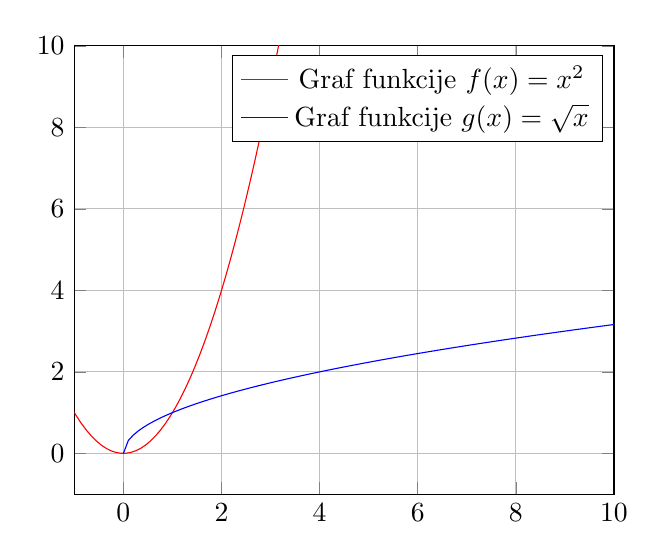
\begin{tikzpicture}
            \begin{axis}[
                grid=major,
                ymin=-1,
                ymax=10,
                xmin=-1,
                xmax=10,
            ]
                \addplot[
                    color = red,
                    samples = 100
                ]{x^2};
                \addlegendentry{Graf funkcije \(f(x) = x^2\)}
                \addplot[
                    color = blue,
                    samples = 100,
                    domain = 0:10
                ]{x^(1/2)};
                \addlegendentry{Graf funkcije \(g(x) = \sqrt{x}\)}
            \end{axis}
        \end{tikzpicture}
        \caption{Graf kvadratne funkcije i korijena na intervalu \(\mathbb{R}^+\)}
        \label{fig:template}
    \end{figure}